\section{问题一求解与分析}
\label{sec:q1}
\subsection{问题的描述与分析}
第一问中，每个子图均作为一个独立执行任务。子图划得过细，虽然容易将计算量分散到多个核心，却增加了任务切换和跨子图搬运；子图过大，又可能压低并行度，并加剧片上存储压力。因此，子图划分、核心归属和核内子图顺序应联合决定。本文用一个完整方案描述三项决策，再以固定执行规则得到总体任务执行时间（Makespan）。后两问保持这一决策空间，通过改变任务边界、交接和缓存规则，解释同一类方案的执行差异。

图~\ref{fig:q1_overview} 概括本问的求解逻辑。先从原始计算图提取依赖、计算负载和张量复用关系，形成若干完整初始方案；再围绕当前可行方案进行互补的邻域改进。便宜的结构条件和下界用于排除明显不合适的候选，完整执行评价决定是否保留候选。最后分别分析核数扩展、逐例差异、搜索过程和可证明的目标界，而非只报告一个平均加速比。
\begin{figure}[htbp]
\centering
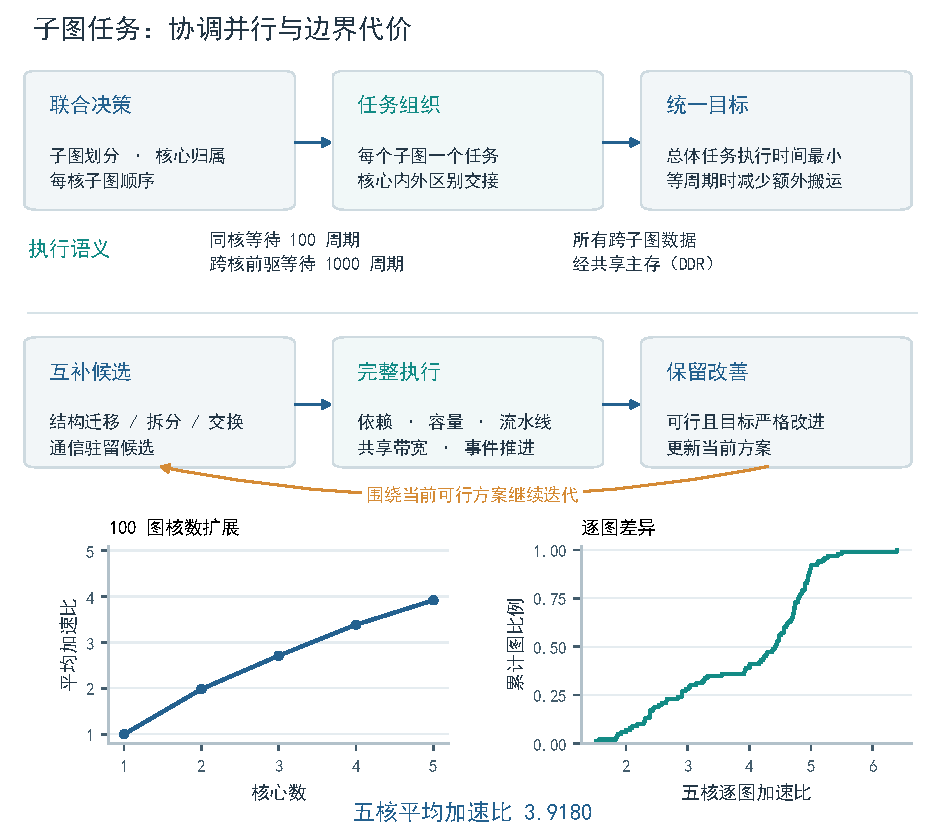
\includegraphics[width=\textwidth]{../求解/问题一/图片/q1_overview.pdf}
\caption{问题一的联合建模与迭代改进框架}\label{fig:q1_overview}
\end{figure}


\subsection{联合决策模型与统一目标}
\subsubsection{计算图、张量与划分}
沿用题面，原始二部有向无环图记为 $G=(T\cup O,E)$，其中 $T$ 为张量集合，$O$ 为操作集合。定义需要分配的非边界搬运算子集合
\begin{equation}
 V=\{o\in O:\operatorname{type}(o)\notin\{\mathrm{COPY\_IN},\mathrm{COPY\_OUT}\}\}.
\end{equation}
原始算子的类型和计算周期、张量大小及依赖关系均保持不变。边界搬运操作由任务划分及执行规则重建。对于张量 $t\in T$，记其大小为 $b_t$，生产者与消费者集合分别为 $P_t$ 和 $C_t$。一个张量被多个算子消费时，不能把它视为彼此独立、没有复用关系的若干份数据。生产者到多个消费者的关系可用有向超边表达；相关无环超图划分研究提供了这种集合表示\cite{A39}。本文仍依据任务边界生成实际搬运，超边连接度只作为候选构造的代理量。

设可用核心集合为 $K=\{1,\ldots,n\}$。完整方案写为
\begin{equation}
 x=(\mathcal P,a,\boldsymbol\pi),\qquad
 \mathcal P=(V_1,\ldots,V_m),\quad a:\{1,\ldots,m\}\longrightarrow K .
 \label{eq:plan}
\end{equation}
其中，$V_i$ 是第 $i$ 个子图包含的算子集合，$a(i)$ 是该子图的核心归属，$\pi_k$ 是核心 $k$ 上子图的执行顺序。划分满足
\begin{equation}
 V_i\ne\varnothing,\qquad \bigcup_{i=1}^{m}V_i=V,\qquad
 V_i\cap V_j=\varnothing\quad(i\ne j).
 \label{eq:partition}
\end{equation}
每个子图恰好出现于一个核心序列且只出现一次，允许部分核心没有子图。因而，核数增大并不强制所有核心都承担工作；它增加可用资源和方案选择空间。

将各 $V_i$ 收缩为顶点，可得到子图依赖商图 $H(\mathcal P)$。再加入各 $\pi_k$ 中相邻子图的顺序边，得到 $H_x$。必要条件为
\begin{equation}
 H_x\text{ 是有向无环图}.
 \label{eq:acyclic}
\end{equation}
仅有原图无环并不能保证任意分组后的商图无环。例如，交错地收集依赖链上不连续的算子，可能在收缩后产生双向依赖。无环划分文献对此给出了明确约束\cite{A02}。本题还存在执行流水线和存储复用关系，所以式~\eqref{eq:acyclic} 用于结构筛选，最终可行性由完整执行确定。

\subsubsection{执行映射与三问的共同方案空间}
记固定配置为 $\theta$，问题编号为 $q\in\{1,2,3\}$。定义执行映射
\begin{equation}
 \mathcal E_q(G,x;\theta)
 =\bigl(\operatorname{feas}_q(x),\mathcal R_q(x),C_q(x),D_q(x)\bigr).
 \label{eq:evaluator}
\end{equation}
$\operatorname{feas}_q$ 表示可行性，$\mathcal R_q$ 为完整执行事件序列。对于重建边界搬运、插入存储换出和取回后得到的操作集合 $J_q(x)$，设操作 $j$ 的开始、完成时刻为 $s_j,f_j$。定义
\begin{equation}
 C_q(x)=\max_{j\in J_q(x)} f_j,
 \qquad x\in\mathcal F_q:=\{x:\operatorname{feas}_q(x)=1\}.
 \label{eq:makespan}
\end{equation}
$C_q$ 即总体任务执行时间（Makespan），单位为周期；$D_q$ 是按题面口径计算的额外 COPY 字节。本文以 $C_q$ 为主目标，周期相同则选择 $D_q$ 较小者，即
\begin{equation}
 \min_{x\in\mathcal F_q}^{\mathrm{lex}}\bigl(C_q(x),D_q(x)\bigr).
 \label{eq:objective}
\end{equation}
这一处理避免为周期和字节引入缺乏物理依据的加权系数。额外 COPY 字节衡量搬运操作规模，不等于某次执行中实际经过 DDR 的全部字节；第三问缓存命中的读请求尤其需要区分这两种统计。

三问均采用式~\eqref{eq:plan} 的决策，改变的是执行映射。记算子 $v$ 所属子图为 $g(v)$，其执行任务标识为
\begin{equation}
 \chi_q(v)=\begin{cases}g(v),&q=1,\\a(g(v)),&q=2,3.\end{cases}
 \label{eq:task}
\end{equation}
这一定义把三问组织为同一模型的三个执行场景：第一问任务随子图划分，第二问任务随核心划分，第三问在第二问基础上增加共享只读缓存。分组、映射和顺序之间的耦合因此始终存在，而不需要为每问重新设计独立目标。

\subsection{第一问的执行、存储与带宽约束}
\subsubsection{任务边界与交接}
第一问一个子图对应一个 Task。同一核心相邻任务之间也需要把边界张量写入 DDR，下一任务再读取，不能把同核跨子图通信直接赋为零。此处与许多任务聚类模型中的同处理器免费通信假设不同\cite{A49}。图~\ref{fig:q1_task} 表示第一问的任务边界与就绪关系。
\begin{figure}[htbp]\centering
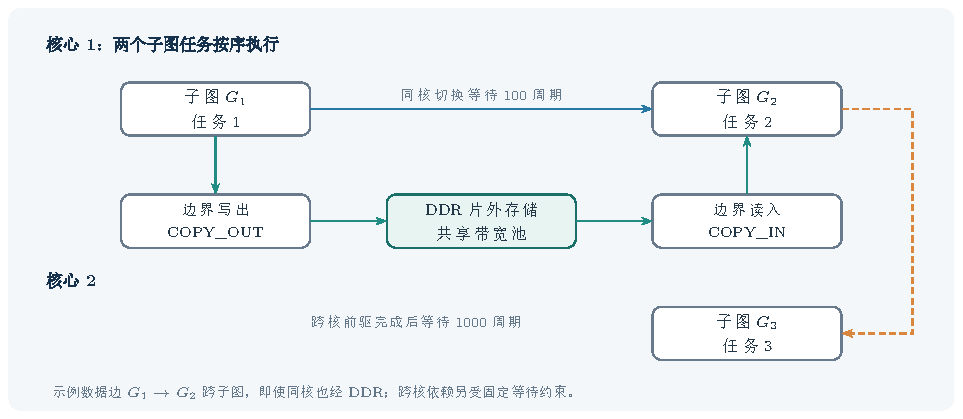
\includegraphics[width=\textwidth]{../求解/问题一/图片/q1_task.pdf}
\caption{子图级任务的边界与交接}\label{fig:q1_task}
\end{figure}

设任务 $i$ 的完成时刻为 $F_i$。任务 $j$ 的启动须同时满足其数据依赖和本核前序任务约束。对相邻本核任务，须有 $S_j\ge F_i+100$；对跨核前驱任务，须有 $S_j\ge F_i+1000$。存在多个前驱时取这些约束的最大值，而不是把所有前驱的等待逐个累加。100 与 1000 均以周期计，搬运本身占用的共享 DDR 服务时间还需单独通过事件执行获得。

任务边界使粒度选择出现双重影响。合并子图可以消除两者之间的一部分任务切换和边界搬运，但也固定了更多算子的共同归核，减少跨核重叠机会。进一步合并还可能延长张量驻留区间，引发自动换出。故单纯最小化边界张量大小，或者单纯均衡算子周期总和，都不足以决定总体任务执行时间（Makespan）。

\subsubsection{固定核内调度与片上容量}
每核具有矩阵、向量、读入和写出四条流水线。每条流水线同时至多服务一个操作；不同流水线可以在满足依赖和容量条件时重叠。算子的开始时刻满足前驱完成、所属流水线可用以及所需片上缓冲可分配等条件。题面规定的核内处理先给出固定操作顺序，再处理存储换出，最后生成流水线依赖。求解变量没有包含任意算子重排、张量重算或自由地址选择。

令 $r\in\{\mathrm{L1},\mathrm{UB}\}$ 表示片上存储区，$B_r$ 为容量；$\mathcal B_{k,r}(\tau)$ 是时刻 $\tau$ 核心 $k$ 在该区已分配且尚未释放的缓冲实例集合。容量条件写为
\begin{equation}
 \sum_{b\in\mathcal B_{k,r}(\tau)}\operatorname{size}(b)\le B_r,
 \quad B_{\mathrm{L1}}=524288\ \mathrm B,\quad B_{\mathrm{UB}}=131072\ \mathrm B.
 \label{eq:capacity}
\end{equation}
式中按实际缓冲实例计量，不能只统计不同逻辑张量的数量。一个逻辑张量在不同核上的驻留副本分别占用相应核心的容量。任务切换还会清除本核任务私有存储，跨任务复用必须经由题设路径完成。

在固定顺序下容量不足时，执行规则依据下一次使用位置选择允许换出的张量，并在后续需要时重新取回。当前操作需要的输入、输出等对象受换出资格限制。该机制属于执行映射的一部分，候选改变划分和顺序后，换出量会随之变化。联合调度与存储优化研究说明了驻留状态对片外访问的重要性\cite{A16}，但其允许的连续地址与自由置换不属于本题决策，因此本文只采用活跃集和驻留压力来解释、提出候选，不移用其优化模型的最优性结论。

\subsubsection{共享 DDR 的事件推进}
设 DDR 总带宽为 $\beta_{\mathrm{DDR}}=60\ \mathrm B/\text{周期}$。对当前在途请求集合 $\mathcal A_D(\tau)$，记 $m_D(\tau)=|\mathcal A_D(\tau)|$。若以独占该带宽所需周期表示请求 $j$ 的剩余服务量 $w_j$，在没有新的发射或完成事件的时间区间内，有
\begin{equation}
 w_j(\tau+\Delta)=\max\left\{0,w_j(\tau)-\frac{\Delta}{m_D(\tau)}\right\},\quad j\in\mathcal A_D(\tau).
 \label{eq:bandwidth}
\end{equation}
整数周期的最小服务长度及舍入按固定执行器处理。新的读写发射、请求完成和任务就绪都会改变下一个事件时刻。事件执行依次处理完成事件，释放依赖和存储，再发射满足条件的新操作。

因此，一次搬运的完成时刻取决于与它重叠的其他请求，不能在优化前固定为一条通信边的常数权重。局部划分即使减少了总搬运字节，也可能改变发射集中程度，进而延迟关键计算链。候选代理适合快速排序，完整执行评价则用于确定真实周期；两者在本文中承担不同作用。

\subsection{下界、候选过滤与质量界}
\subsubsection{对全体方案有效的下界}
取所有可行方案都保留的计算依赖图 $G_c$，其中算子 $v$ 的固定服务周期为 $p_v$，计算流水线类型为 $\rho(v)$。定义计算路径、流水线负载和必要 DDR 流量下界：
\begin{align}
 L_{\mathrm{path}}&=\max_{P\text{ 为 }G_c\text{ 中依赖路径}}\sum_{v\in P}p_v,\\
 L_{\mathrm{load}}&=\max_r\frac{\sum_{v:\rho(v)=r}p_v}{n},\\
 L_{\mathrm{DDR}}&=\frac{B_{\mathrm{mandatory}}}{\beta_{\mathrm{DDR}}},\qquad
 L=\max\{L_{\mathrm{path}},L_{\mathrm{load}},L_{\mathrm{DDR}}\}.
 \label{eq:lower}
\end{align}
$B_{\mathrm{mandatory}}$ 只包含能证明所有方案都必须通过 DDR 服务的字节。对第一、二问，初始输入读取和最终输出写出提供这种必要流量；第三问的初始缓存为空，无逻辑别名时首次读取仍须经过 DDR。若存在可能影响首次读取计数的显式逻辑别名，则对第三问保守去掉这一读下界，保留必要写出量。

\textbf{命题1：}在计算依赖保留、算子不重算或删除、同类计算流水线每核串行、必要 DDR 流量判断成立的条件下，对任意可行方案 $x$，有 $L\le C_q(x)$。

\textbf{证明：}同一计算依赖路径上的算子只能依次完成，故执行周期不小于任意路径的计算服务量之和。每种计算流水线在 $n$ 个核心上的总能力为每周期至多提供 $n$ 个流水线周期，因此其总工作量除以 $n$ 不大于执行周期。DDR 在任意长为 $C_q(x)$ 的区间内至多服务 $\beta_{\mathrm{DDR}} C_q(x)$ 字节，必要流量又给出第三项约束。三项分别成立，取最大值仍为下界。计算与搬运可以重叠，因此不能将三项直接相加。证毕。

\subsubsection{固定候选的下界}
固定完整候选 $x$ 后，归核已经确定，可进一步计算每个核心各类流水线的工作量下界。第一问还可以在任务依赖和核心顺序合图上，按每个任务的计算负载下界及对应交接等待递推最早完成下界。设任务 $i$ 的工作下界为 $\ell_i$，前驱集合为 $\operatorname{pred}_x(i)$，交接等待为 $d_{hi}$，则
\begin{equation}
 z_i=\ell_i+\max_{h\in\operatorname{pred}_x(i)}(z_h+d_{hi}),
 \label{eq:taskbound}
\end{equation}
无前驱时最大项取零。$\ell_i$ 取该任务各计算流水线总负载的最大值，允许流水线充分重叠；$d_{hi}$ 只使用题设确实要求的任务等待。由拓扑序归纳可知，真实任务完成时刻不早于 $z_i$。把这些项以及固定任务边界产生的必要搬运下界取最大值，得到候选专属下界 $L(x)$。

\textbf{命题2：}若 $L(x)\le C_q(x)$，当前已保留方案周期为 $U$，则 $L(x)>U$ 的候选不能改善主目标。

\textbf{证明：}$C_q(x)\ge L(x)>U$，故该候选的周期严格更差。证毕。过滤使用严格大于；当 $L(x)=U$ 时，候选仍可能在相同周期下减少额外 COPY 字节。候选下界只对固定的 $x$ 有效，不能作为整个方案空间的最优值下界。

\subsubsection{可行上界与相对差距}
令 $C_q^*$ 为全局最优周期，当前可行周期为 $U$。当 $0<L\le C_q^*\le U$ 时，
\begin{equation}
 0\le\frac{U-C_q^*}{U}\le1-\frac{L}{U},\qquad
 0\le\frac{U}{C_q^*}-1\le\frac{U}{L}-1.
 \label{eq:gap}
\end{equation}
第一式量化相对于当前方案仍可能减少的比例，第二式以最优值为分母；二者不能互换。本文以第一式右侧作为近界停止依据，当其不超过 $0.0025$ 时停止继续改进。其他停止原因只表示预算或搜索机会用尽，不说明式~\eqref{eq:gap} 已经很小。

\subsection{多邻域迭代改进算法}
\subsubsection{初始构造与当前可行方案}
初始方案来源包括同配置的已有可行方案、依赖关键性引导的构造及按负载和图结构形成的划分。已有方案先在当前配置下得到有效执行结果，随后才作为当前解。构造中使用的上行优先级与最早完成位置思想可追溯到经典列表调度\cite{A01}，但本题的共享 DDR 和任务边界决定了该估计只能用于提出候选。

不同构造重视的结构并不相同：链相关的算子倾向共同归核，较宽的独立分支提供并行机会，细粒度阶段划分则为后续迁移和合并保留调整空间。算子间调度研究也指出，分组与并行执行策略共同决定收益\cite{A08}。本文没有改变原始算子图，而是在允许提交的三个变量上组织这些构造。若已有较少核心的有效方案，可以增加空核心后作为当前核数的候选，再由当前配置评价，而不强行把其子图拆到所有核心。

\subsubsection{互补候选及父方案更新}
在当前完整方案周围，采用以下互补方式产生候选。结构候选通过子图迁移、相邻交换、前缀拆分及联合迁移调整并行度和交接；驻留候选分析张量消费者集合、活跃区间和生产者释放位置，提出共同归核或局部顺序变化；基础构造保留不同阶段粒度和前沿划分的探索。第三问还开放基于缓存事件的纯顺序候选，其机制在第~\ref{sec:q3} 节说明。

每个候选均输出式~\eqref{eq:plan} 的完整对象，不只提交一个无法独立评价的局部增量。保留新当前方案后，依赖父方案的局部候选流重新基于该方案建立；不依赖父方案的全局构造保留原有进度。这样既使局部搜索适应已经取得的改进，又避免在每次接受候选后重复从头生成相同的全局方案。相同完整方案只保留一次评价机会。

多初值与可行解上的局部迁移是现实多处理器调度中常用的改进组织\cite{A42}。本文采用这一通用思想，但所有接受判断都在本题事件模型下进行，不使用其他调度模型的代价替代本题周期。

\subsubsection{来源选择与有限预算}
候选生成和完整评价的成本差异较大，因此按近期反馈分配搜索机会。设来源 $a$ 最近的相对周期改进均值为 $\bar g_a$，生成与评价总用时的近期中位数为 $\widehat c_a$，失败比例为 $r_a$，该来源已完成调用数为 $N_a$，总完成调用数为 $N$。在预热、可用性和剩余时间准入条件满足后，比较指数
\begin{equation}
 I_a=\frac{\bar g_a+0.012\sqrt{\log(2+N)/(1+N_a)}}{
 \max(0.005,\widehat c_a)(1+r_a)}.
 \label{eq:sourcepriority}
\end{equation}
近期统计窗口为最近八次调用。前项奖励已观察到的改进，第二项为尚未充分尝试的来源保留机会，分母计入运行成本和失败倾向。搜索资源根据测量反馈分配的思路与程序自动调优中的经验一致\cite{A12}；式~\eqref{eq:sourcepriority} 是本方法的启发式，不附带概率置信界或遗憾保证。

初期优先覆盖可用来源，间隔过久未调用的来源获得再次尝试机会。按 $1.2\widehat c_a+0.05$ 秒估计准入成本，预计无法在剩余时间内完成时不启动该次评价。每个图、问题和核数配置设置最多 600 秒和 2048 次评价。第三问从总预算中预留同方案无 L2 配对时间。除近界停止外，候选耗尽、预算结束，或至少 30 秒没有周期改善且累计停滞条件满足时停止。保存过程消耗的时间也计入可用解出现时刻。

\subsubsection{可行性保持与目标单调性}
\textbf{命题3：}若初始方案 $x^{(0)}\in\mathcal F_q$，每次只在相同配置下接受完整执行可行且字典序严格改善的候选，则所有已保留方案均可行，且目标序列字典序单调不增。

\textbf{证明：}初始方案可行。第 $k$ 步若没有接受新候选，则保留 $x^{(k)}$；若接受 $y$，其已通过完整执行且 $\bigl(C_q(y),D_q(y)\bigr)<_{\mathrm{lex}}\bigl(C_q(x^{(k)}),D_q(x^{(k)})\bigr)$，因此 $x^{(k+1)}=y$ 可行且严格改善。由归纳法得结论。证毕。

这一性质针对实际保留的方案，不能把未完成评价的候选、未保存成功的终值或搜索代理曲线当作已取得解。有限方案空间结合严格接受和去重限制了重复改进，实际实现还受有限时间、调用次数及停滞条件约束。算法终止不等于全局最优；质量界只在有效全局下界及可行上界均存在时使用。

\subsection{联合迭代的计算过程}
\subsubsection{从完整方案到一次可接受的改进}
第~\ref{sec:q1} 节给出了方案空间、全局下界和接受准则。本节把候选从生成到保存的计算顺序具体化。对一个固定的计算图、问题编号和核数，搜索状态包含已验证的当前最好方案 $x$、对应完整执行结果、父方案代号、已经评价或安全剪枝的完整方案集合，以及各候选来源的近期记录。这里“当前最好”只有一个；不同来源产生的候选都与这个状态比较，来源自身不保存另一套最终解。初始构造可以来自本配置下已经验证的完整方案，或由依赖关键性、阶段粒度与负载映射生成。对初始候选先做结构检查，再取得完整执行结果；只有合法结果才进入当前最好状态。

一次迭代可按下列顺序表述，其中 $U=C_q(x)$，$L(y)$ 是固定候选 $y$ 的有效周期下界：
\begin{enumerate}
  \item 根据仍可用的来源、近期改善幅度、生成与评价成本、失败比例及剩余时间选择一个来源。初次覆盖和久未访问的来源获得机会；预计成本超过剩余时间时停止准入。
  \item 来源提出完整候选 $y=(\mathcal P',a',\boldsymbol\pi')$。检查非边界算子覆盖、每个子图恰有一次归核及商图与核内顺序合图的无环性；相同完整方案不重复评价。
  \item 若 $L(y)>U$，该候选不可能改善主目标，直接筛去。等号情形保留，因为周期持平时额外 COPY 字节仍可能下降。
  \item 对其余候选调用完整执行，重建任务和边界搬运、自动换出、Pipe 排布与共享带宽事件。只有结果可行，且 $(C_q(y),D_q(y))<_{\rm lex}(C_q(x),D_q(x))$，才令 $x\leftarrow y$ 并更新父方案代号；取得的解在评价和保存完成后才计为可用。
  \item 检查全局下界相对差距、评价次数、墙钟预算、来源耗尽和停滞条件。第三问结束主搜索后，对已选同一方案另作无缓存评价，配对结果不参与主搜索的接受判断。
\end{enumerate}
选择来源的反馈指数见式~\eqref{eq:sourcepriority}。实际准入先考虑少量来源预热与时间可行性，再比较近期收益和成本；它是调配有限评价机会的规则，不是候选周期的替代预测。每次接受都会改变父方案，故候选生成必须明确绑定接受前的状态。例如驻留候选使用先前的张量生命周期，缓存候选使用先前的读入与淘汰事件；若父方案改变，继续消耗旧候选流可能把旧事件错误关联到新划分或新归核。实现因此在新父方案代号出现后重建依赖父方案的结构、驻留和缓存流，并以已接受的完整方案及执行记录为起点。与父方案无关的全局构造流则保存其迭代位置，避免每次改进后重新生成相同初值。这个区分也解释了为何来源调用数不能直接看作互不干扰的独立实验。

\subsubsection{邻域更新、结构预检与计算量}
令 $N=|V|$ 为需归组的非边界算子数，$M$ 为这些算子间保留的依赖边数，$m$ 为当前子图数，$H(y)$ 为候选 $y$ 的完整执行实际处理的事件数。一次“迁移”把一个完整子图从原核心序列删除，再插入目标核心序列的某个合法位置；它更新 $a$ 与相关的 $\pi_k$，但不改变该子图内部算子集合。“交换”改变两个子图在一个或两个核心序列中的相对位置；若跨核交换，还同时更新两者归属。“拆分”把某子图分成非空、互不相交的两部分，在算子到子图映射中为新部分赋编号，并重新安置两部分的核心位置与先后顺序。联合迁移及张量关联移动按依赖闭合的子图集合操作，其输出仍须含全部 $N$ 个算子的完整映射和各核序列。拆分后的新增边界搬运、迁移后的跨核通信以及顺序变化造成的驻留区间，均由新方案的执行结果计算，不能从旧目标值直接加减。

给定一个已经构造好的完整候选，扫描 $N$ 个算子建立组成员与归属，扫描 $M$ 条依赖建立跨组前驱，再加入各核相邻子图的顺序边。后者总数不超过 $m$；在合图上做一次拓扑检查，按通常邻接表实现，其工作量为 $O(N+M+m)$，存储量同阶。这只是必要的结构预检复杂度，不是完整求解复杂度。环检查能够排除“某组必须先于另一组、又被核内顺序要求后于另一组”的矛盾，却不能决定瞬时缓冲是否可分配、自动换出是否引入额外请求、任务等待如何落在时间轴上，以及共享带宽在并发请求间如何分配。因此，通过预检的候选仍须完整执行验证。对事件评价记其实际成本为 $T_{\rm eval}(N,M,m,H(y))$；仅因事件轨迹含 $H(y)$ 项，不能未经实现级证明便称该成本对 $H$ 或 $N$ 线性。

候选空间本身也远大于一次预检。只枚举单个子图向其他核心迁移，已有至多 $m(n-1)$ 种归核选择；再考虑每个目标核心的插入位置、两个子图交换、组内依赖合法的拆分、多个关联组联动，候选数会继续增加。完整执行还有固定方案生成的 COPY、Spill 和 FIFO 事件，$H(y)$ 由候选实际轨迹决定，不能预先用原图边数替代。实际程序对单次来源流设生成上限，整配置最多评价 $2048$ 次，并以 $600$ 秒总预算及剩余时间准入约束搜索。若实际完成 $B$ 次评价，总代价应写成各次生成、结构检查、保存及 $\sum_{i=1}^{B}T_{\rm eval}(N,M,m_i,H_i)$ 的和，而非一个脱离候选数与轨迹长度的单一线性式。搜索中的下界剪枝、去重和早停减少实际调用，却不把有限预算算法变为全局枚举。

\subsubsection{两张五核图的方案展开}
真实五核方案能够说明“子图数”与“执行任务数”在两问中的差别。图80在第一问选出 $3$ 个子图，核心序列长度为 $(1,1,1,0,0)$：五个核心可用，但只有三个核心承担工作，三个子图分别构成 Task，最终总体任务执行时间为 $100325$ 周期，额外 COPY 为 $3047424$ B。第二问对同图独立寻优后得到 $161$ 个子图，五核序列长度为 $(34,32,34,30,31)$，周期为 $71369$，额外 COPY 为 $2273280$ B。第二问仍有许多子图，却只有五个核心级 Task；同核子图可延续存储状态，跨核交接按写出完成后等待的规则执行。由于两问同时改变了划分、归核和顺序，这组周期差只说明各自选中方案的表现，不能当作固定方案下删除任务等待的净效果。

图46的第一问五核方案含 $15$ 个子图，序列长度为 $(4,2,2,2,5)$。每个子图是独立 Task，所以五核序列中共有 $15-5=10$ 处同核相邻 Task 交接；承担五个子图的核心至少经历四次按题设定义的相邻任务等待。该方案周期为 $91730$，额外 COPY $3669568$ B，其中划分搬运 $3564096$ B、自动换出 $105472$ B。第二问独立选出的方案含 $31$ 个子图，序列长度为 $(5,7,7,5,7)$，周期 $69268$，额外 COPY $2469536$ B，未产生自动换出的额外字节。虽然第二问有更多子图，其同核子图不构成新的 Task 边界；第一问同核相邻 Task 的等待也不能简单乘以十再从 $91730$ 中相减，因为五核并行执行、跨核依赖和 DDR 服务会使这些等待与其他事件在时间上交错。两例分别展示了有效核心数、子图粒度和自动换出如何与任务规则共同进入完整周期。

\subsubsection{可行方案空间的嵌入性质}
现有下界说明任一可行结果距离全局最优最多仍可能改善多少。另有一项与核数有关、但不依赖搜索启发式的性质。固定问题编号和全部硬件参数，设允许核心空闲，增加一颗核心不减少原核心的 Pipe、L1/UB 容量，也不改变共享 DDR 或 L2 总带宽与事件优先规则。对任意 $n$ 核可行方案 $x$，构造 $n+1$ 核方案 $\iota(x)$：保持全部子图集合、算子映射、原有核心归属及原核序列不变，仅令新增核心的序列为空。由于没有任何新操作、COPY 或缓存请求从空核心发射，原方案的任务边界、缓冲实例和事件顺序均不变，故
\begin{equation}
 \iota(x)\in\mathcal F_q(n+1),\qquad
 C_q(\iota(x))=C_q(x),\qquad D_q(\iota(x))=D_q(x).
 \label{eq:core_embedding}
\end{equation}
于是同配置、同评价规则下的理论最优周期满足 $C_{q,n+1}^{*}\le C_{q,n}^{*}$。证明只需把任意 $n$ 核可行方案按上法嵌入 $n+1$ 核可行集；后者的最小值不大于其中这个方案的周期。该命题不要求新增核心必须被使用，也不意味着增加核心必然严格缩短周期。实际有限预算算法分别搜索不同核数，其已找到的两个方案并不构成包含关系；来源准入、候选顺序和搜索截止可能不同，所以观察到的近似结果不能单凭式~\eqref{eq:core_embedding} 声称逐图随核数严格单调。第一、二问的一核点还采用题设约定的原始整图参考，跨这一特殊基准解释时应使用实际统一评价定义，而不是把约定点误作上述嵌入构造的搜索输出。


\subsection{实验指标与第一问结果}
\subsubsection{统一评价与核数扩展}
实验使用题面提供的 100 个计算图及固定参数，统一以周期评价。对图 $i$，记原始整图单核周期为 $T_{i,0}$，本问 $n$ 核方案周期为 $C_{i,1,n}$，定义
\begin{equation}
 S_{i,q,n}=\frac{T_{i,0}}{C_{i,q,n}},\qquad
 \overline S_{q,n}=\frac{1}{100}\sum_{i=1}^{100}S_{i,q,n}.
 \label{eq:speedup}
\end{equation}
第一、二问的一核点按题设为 1。平均加速比先逐图求比再取算术平均，而不是先对周期求和再求比。后一种做法会按原始周期给大图更高权重，回答不同的评价问题。

% 由求解/规范化数据/combined/means.csv 生成；逐图加速比的算术平均。
\begin{table}[htbp]
\centering\small
\setlength{\tabcolsep}{5pt}
\begin{tabular}{rrrrrr}
\toprule
核心数 & 样本数 & 平均加速比 & 中位加速比 & 最小加速比 & 最大加速比 \\
\midrule
1 & 100 & 1.0000 & 1.0000 & 1.0000 & 1.0000 \\
2 & 100 & 1.9832 & 1.9810 & 1.2445 & 3.6480 \\
3 & 100 & 2.7106 & 2.8440 & 1.4596 & 5.4659 \\
4 & 100 & 3.3852 & 3.7003 & 1.5139 & 6.3806 \\
5 & 100 & 3.9180 & 4.4227 & 1.5157 & 6.3928 \\
\bottomrule
\end{tabular}
\caption{问题一各核数逐图加速比统计}\label{tab:q1_mean}
\end{table}

图~\ref{fig:q1_mean} 和表~\ref{tab:q1_mean} 给出核数扩展结果。五核平均加速比为 $3.9180$，中位数为 $4.4227$。由四核增加至五核仍有收益，但平均增量小于低核数阶段，反映依赖串行部分、任务交接及共享带宽对进一步并行的限制。
\begin{figure}[htbp]\centering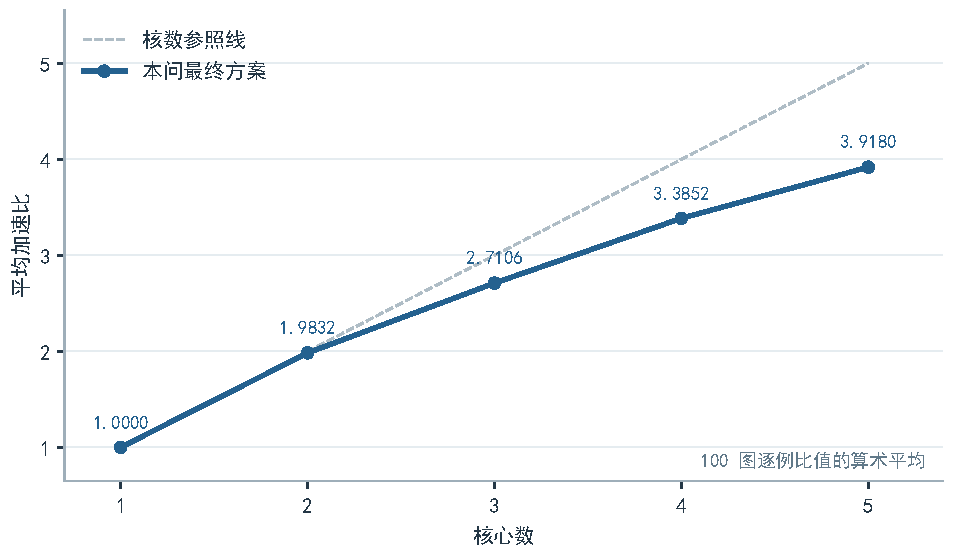
\includegraphics[width=.90\textwidth]{../求解/问题一/图片/q1_mean.pdf}
\caption{第一问各核数平均加速比}\label{fig:q1_mean}\end{figure}

\subsubsection{逐例分布及低收益图}
图~\ref{fig:q1_distribution} 展示二至五核加速比的经验分布。五核配置下，100 个图的加速比介于 $1.5157$ 与 $6.3928$，其中 6 个图低于 2，9 个图超过 5。均值低于中位数，说明少数低收益图对总体平均值有明显影响。仅说明大多数图接近五倍不足以描述完整分布。
\begin{figure}[htbp]\centering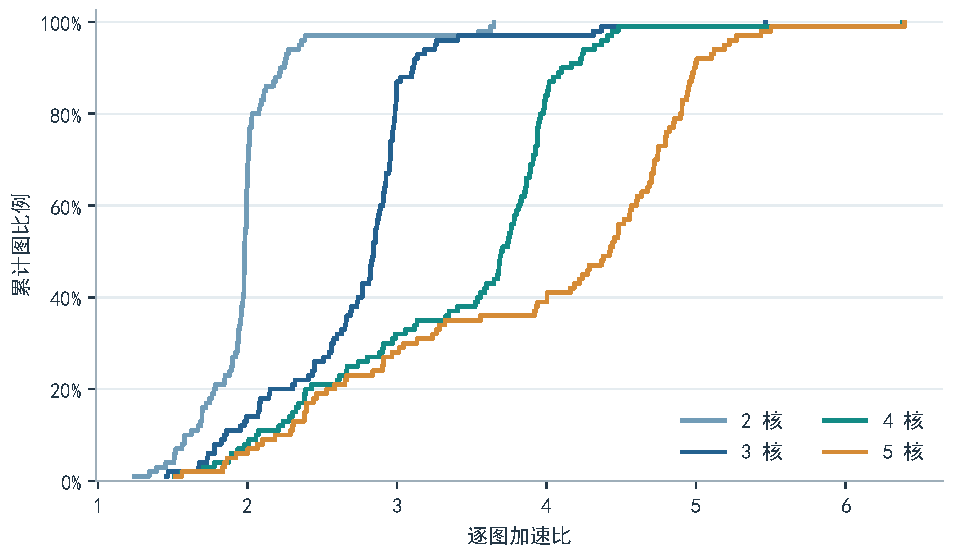
\includegraphics[width=.90\textwidth]{../求解/问题一/图片/q1_distribution.pdf}
\caption{第一问各核数加速比的逐例分布}\label{fig:q1_distribution}\end{figure}

超过核数的加速比不表示计算资源超过了题设。分组和执行顺序可能同时改变自动换出和流水线重叠，使被比较的单核参考与多核方案不再只有核心数量的差别。因此，理想线性加速 $S=n$ 是直观参考，不是这里的普遍性能上界。反之，收益偏低也不能只归因于核负载不均衡，必须结合保留依赖链、任务边界和搬运争用解释。

本问五核额外 COPY 字节的均值为 $14585335.66$ B，中位数为 $1990466$ B，差异说明搬运规模具有明显长尾。88 个五核结果未产生自动换出的额外 COPY，另外的存储压力样本不应被零换出的多数掩盖。本文同时保留逐例周期、划分新增搬运及自动换出子项，以支持对计算和存储瓶颈的区分。

\subsubsection{任意时刻可用解与搜索过程}
设 $\tau$ 为本次搜索累计用时，$\mathcal A(\tau)$ 为在该时刻前已经完整评价并保存的可用候选集合。定义
\begin{equation}
 U(\tau)=\min_{x\in\mathcal A(\tau)}C_q(x).
 \label{eq:anytime}
\end{equation}
若 $\mathcal A(\tau)$ 为空，该采点记为尚无可用解；不得由后来的终值补填。算法停止后，已经保存的解继续可用，所以随后采点可以保持停止时的当前解。图~\ref{fig:q1_anytime} 按每 30 秒原采点展示五核逐例搜索轨迹，颜色表示相对于最终周期的额外比例，未取得可用解的位置单独标识。
\begin{figure}[htbp]\centering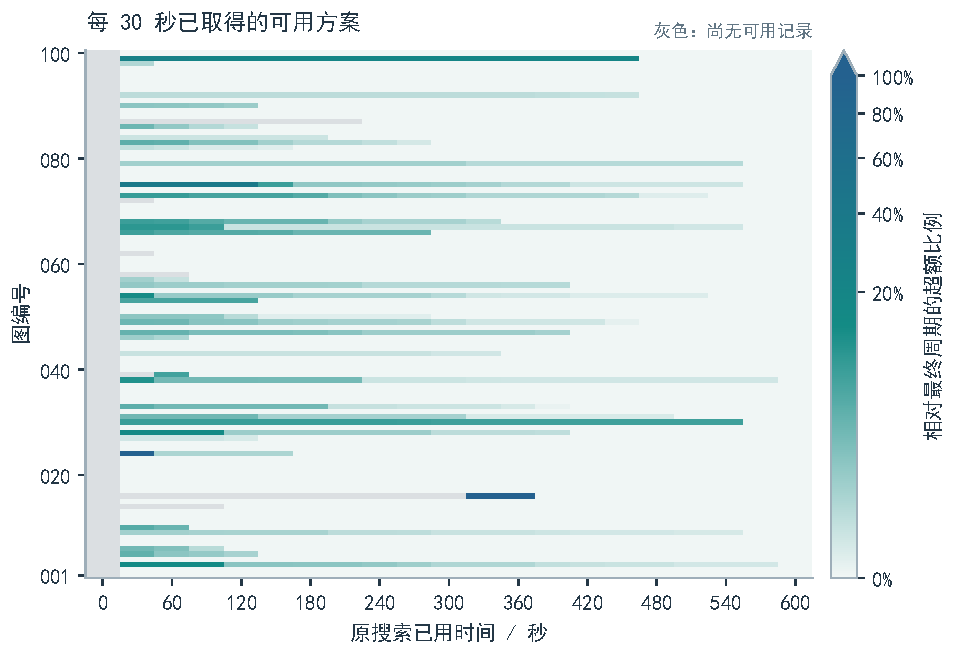
\includegraphics[width=\textwidth]{../求解/问题一/图片/q1_anytime.pdf}
\caption{第一问五核每30秒可用解轨迹}\label{fig:q1_anytime}\end{figure}

该图比较的是一次已给初始资料的改进过程，纵向设备周期与横向主机秒数是不同量纲。算法会根据图结构和来源表现提前结束，故不能将所有水平保持段解释为持续运行但没有改善。阶段统计与停止原因用于解释搜索何时耗尽候选、何时受到剩余时间约束；曲线只反映当时真正可用的方案。

\subsubsection{下界与结果解释}
图~\ref{fig:q1_bound} 对照五核结果周期及全局下界。下界接近结果时，继续搜索能够带来的相对周期减少受到式~\eqref{eq:gap} 约束；下界较松时，较大的差距既可能来自方案质量，也可能来自松弛模型没有刻画任务交接、容量和带宽竞争。不能把松弛差距直接解释成算法实际损失。
\begin{figure}[H]\centering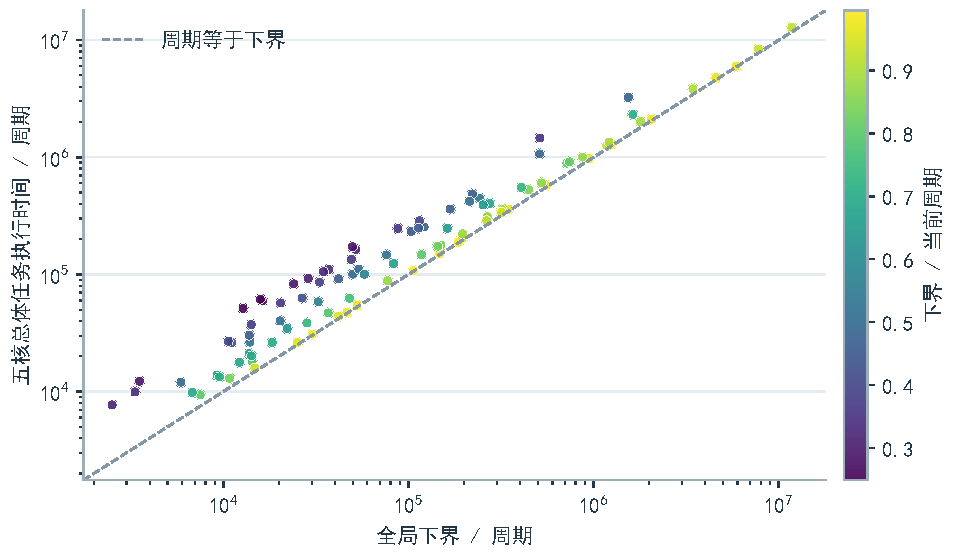
\includegraphics[width=.92\textwidth]{../求解/问题一/图片/q1_bound.pdf}
\caption{第一问五核可行周期与全局下界}\label{fig:q1_bound}\end{figure}

本问建立了后两问共同使用的决策、执行和接受框架。结果表明，联合改变划分、归核和顺序能够获得稳定的多核收益；其边际收益与任务边界的代价相关。第二问保持相同目标，进一步研究任务边界改为核心后，片上驻留与更细粒度跨核交接对这些结果的影响。
